\documentclass[12pt,a4paper]{article}
\usepackage[utf8]{inputenc}
\usepackage[left=2.5cm,right=2.5cm,top=3cm,bottom=2cm]{geometry}
\author{Pauline Speckmann}
\usepackage{graphicx}
\usepackage{booktabs}

\usepackage{fancyhdr}
\pagestyle{fancy}
\fancyhf{}
\fancyhead[l]{Digitalisierung Vorlesung 3 $-$ Zusammenfassung von Pauline Speckmann}
\fancyhead[r]{\thepage}

\begin{document}
\setcounter{section}{2}
\section{Management von Informationssystemen}


\vspace*{1cm}
\subsection{Integrationsorientierte Informationssysteme} %%%%%%%%%%%%%%%%%%%%%%%%%%%%%%%%%%%%%%%%%%%%%%%%%%%%%%%%%%%%%%%%%%%%%%%%
\begin{itemize}
   \item \textbf{Digitaler Zwilling}:\\
         Digitale Darstellung eines realen Objekts oder Systems (materiell oder immateriell)

   \item \textbf{Integrationsansätze}
      \begin{itemize}
			\item \textbf{Datenintegration}:\\
			      Datenbestände von mehreren Informationssystemen werden zentral gespeichert (nicht mehrfach)
			\item \textbf{Funktionsintegration}:\\
			      Mehrere Funktionen werden in einem Informationssystem gebündelt
			\item \textbf{Prozess- oder Vorgangsintegration}:\\
			      In einem Prozess aufeinander folgende Funktionalitäten sind über ein Informationssystem nahtlos miteinander verbunden (Schnittstellen)
		\end{itemize}

   \item \textbf{SAP}: Global führender Anbieter von ERP-Systemen\\
         Beispiel: Verarbeitung eines Kundenauftrags
      \begin{enumerate}
			\item Kundenauftrag wird erfasst
			\item Automatisches Ausführen von: Bestellung der Rohmaterialien, Erzeugung von Fertigungsaufträgen, Übermittlung an die Finanzplanung
			\item Rollen \& Rechte verteilen
      \end{enumerate}

   \item \textbf{ERP- (Enterprise-Ressource-Planning) Systeme}:\\
         Integrierte betriebswirtschaftliche Softwarelösungen, die eine Vielzahl Geschäftsprozesse eines Unternehmens abdecken
      \begin{itemize}
			\item Hohe Datenintegration: Zentrale Datenbank
			\item Hohe Funktions- und Prozessintegration: Schnittstellen
      \end{itemize}
   \item[] 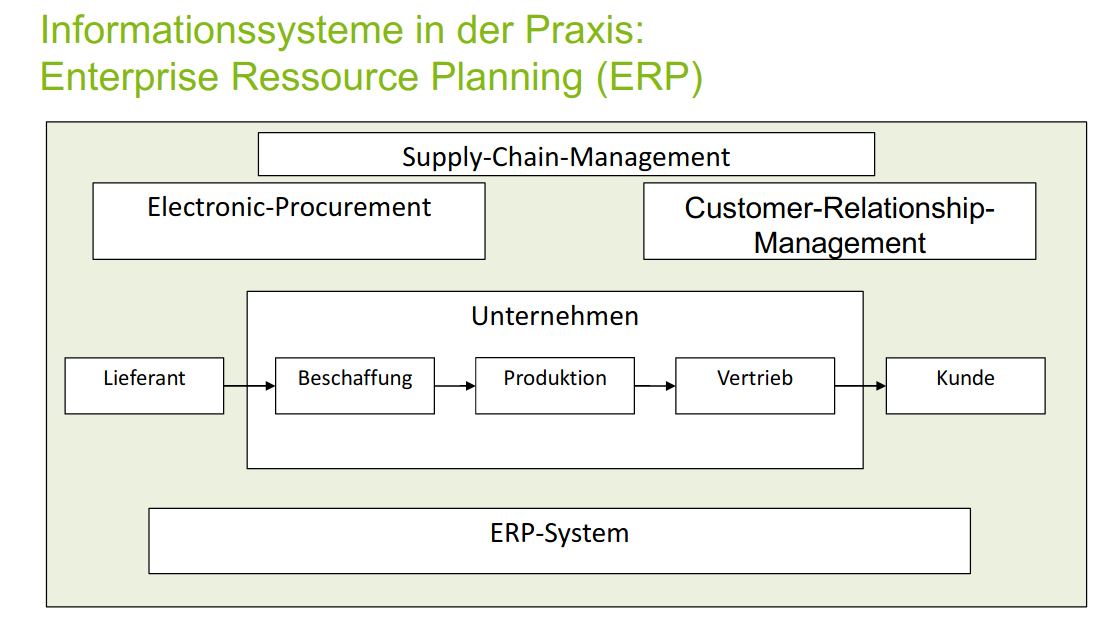
\includegraphics[scale=0.35]{digi_pic.png}
\end{itemize}


\vspace{0.5cm}
\subsection{Auswahl von Informationssystemen} %%%%%%%%%%%%%%%%%%%%%%%%%%%%%%%%%%%%%%%%%%%%%%%%%%%%%%%%%%%%%%%%%%%%%%%%%%%%%%%%%%%
\begin{itemize}
   \item \textbf{Systembereitstellung $–$ Goldene Regeln}:
   \item[] 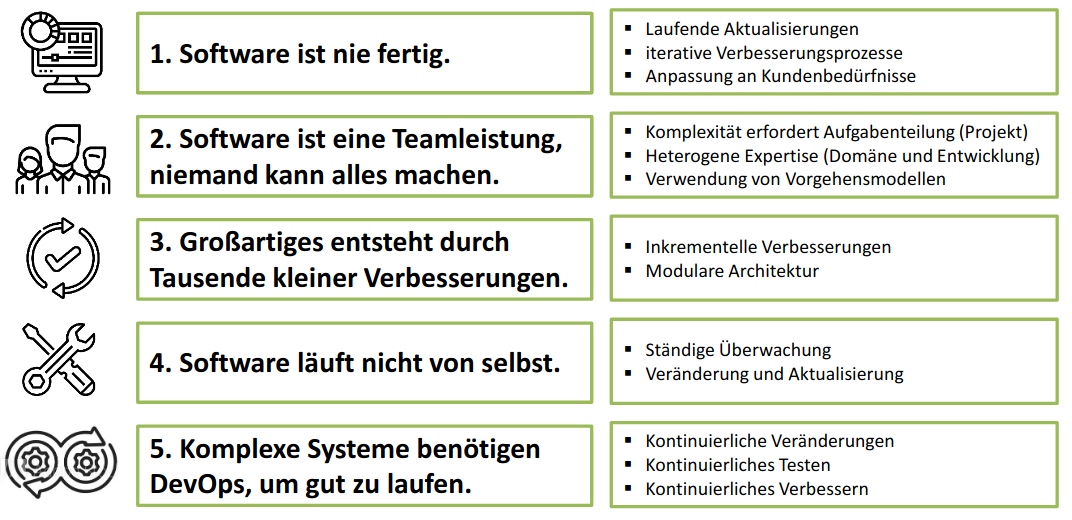
\includegraphics[scale=0.52]{GoldeneRegeln.png}
   
   \item \textbf{Softwareindustrie}:
      \begin{itemize}
			\item Direkte und Indirekte Netzeffekte:\\
			      Der Nutzen eines Programms für einen einzelnen Kunden steigt häufig mit der Gesamtzahl der Nutzer.
			\item Keine Vervielfältigungskosten:\\
			      Hohe initiale Entwicklungskosten, anschließend jedoch nahezu kostenfreie Ver\-viel\-fält\-ig\-ungs\-mög\-lich\-keit\-en (Fixkostendegression)
			\item Kein Wertverlust durch Gebrauch
			\item Make or buy?
         \item[] 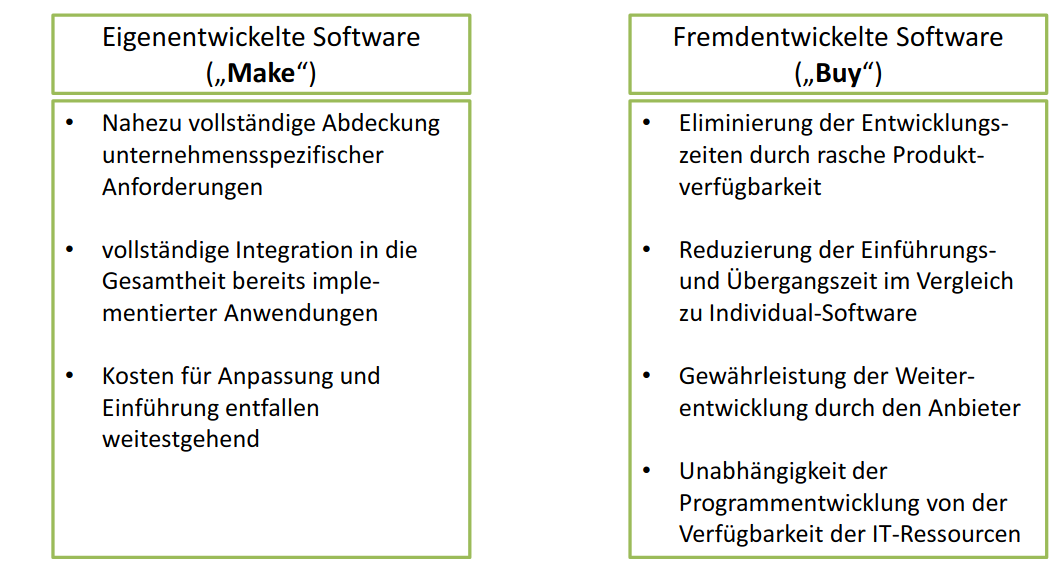
\includegraphics[scale=0.5]{MakeOrBuy.png}
%         \item[] \begin{minipage}[t]{0.43\textwidth} \vspace*{0cm}
%                     \begin{center}
%                        \textbf{Make}:\\
%                        Eigenentwickelte Software
%                     \end{center}
%                     \begin{itemize}
%                        \item Nahezu vollständige Abdeckung unternehmensspezifischer Anforderungen
%                        \item Vollständige Integration in die Gesamtheit bereits implementierter Anwendungen
%                        \item Kosten für Anpassung und Einführung entfallen weitestgehend
%                     \end{itemize}
%                  \end{minipage}
%                  \begin{minipage}[t]{0.45\textwidth} \vspace*{0cm}
%                     \begin{center}
%                        \textbf{Buy}:\\
%                        Fremdentwickelte Software
%                     \end{center}
%                     \begin{itemize}
%                        \item Eliminierung der Entwicklungszeiten durch rasche Produktverfügbarkeit
%                        \item Reduzierung der Einführungs- und Übergangszeit im Vergleich zu Individual-Software
%                        \item Gewährleistung der Weiterentwicklung durch den Anbieter
%                        \item Unabhängigkeit der Programmentwicklung von der Verfügbarkeit der IT-Ressourcen
%                     \end{itemize}
%                  \end{minipage}


\newpage %Manuelle Formatierung
         \item \textbf{Kostenvergleichsrechnung}:
         \item[] 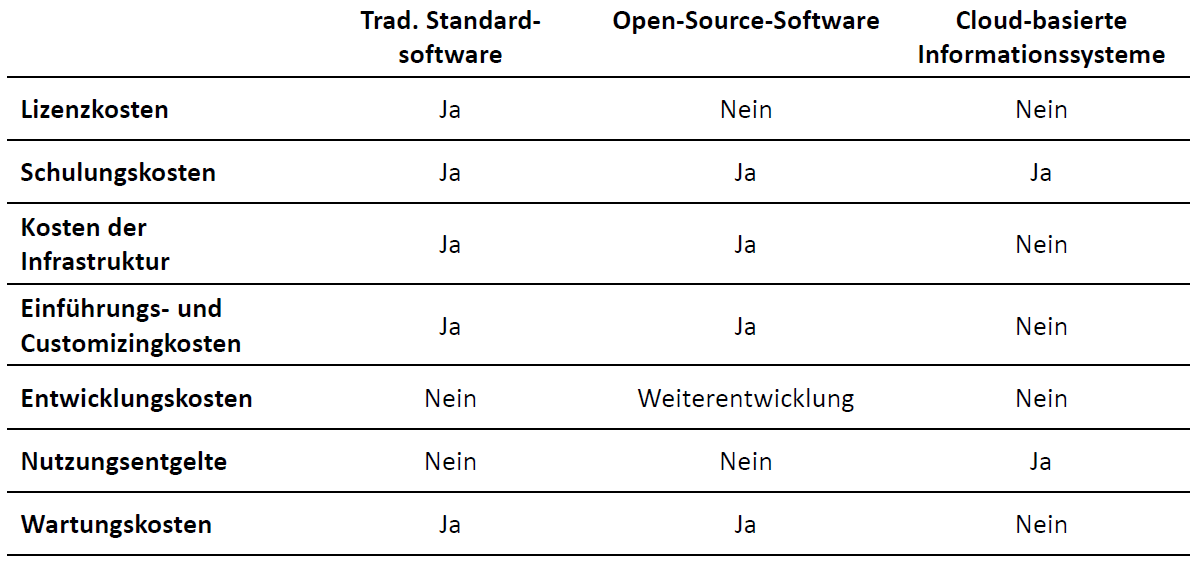
\includegraphics[scale=0.4]{Vergleichskosten.png}         
         
         \item \textbf{Nutzenkategorien von Informationssystemen}:
         \item[] 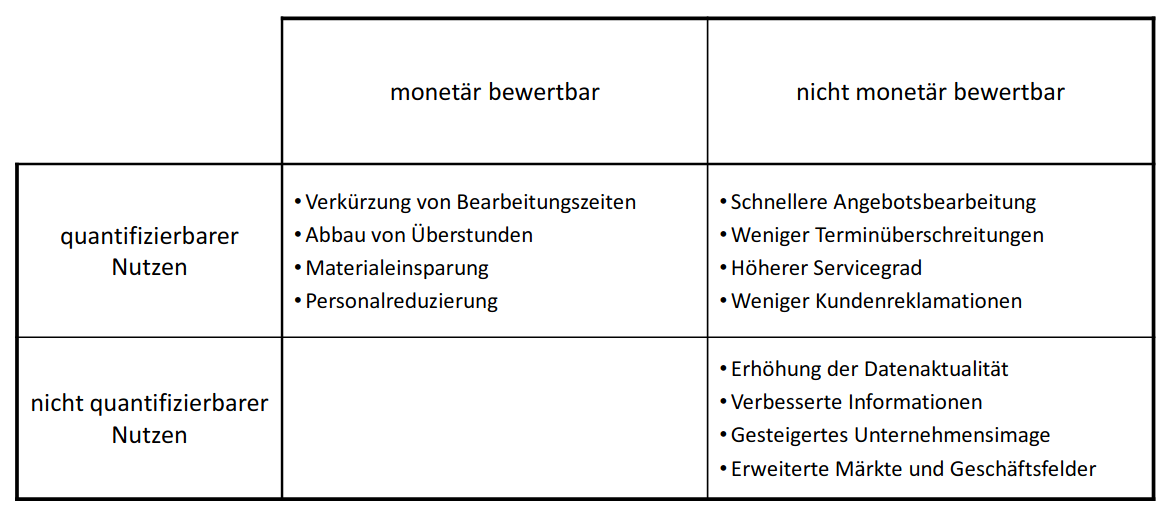
\includegraphics[scale=0.45]{Nutzen.png}
      \end{itemize}
   
   \item \textbf{Anwendungslebenszyklus}:\\
      \begin{minipage}[t]{0.3\textwidth}\vspace*{0cm}
         \begin{enumerate}
				\item Entwicklung
				\item Einführung
				\item Wachstum
				\item Sättigung / Reife
				\item Rückgang
				\item Abschaffung
         \end{enumerate}
      \end{minipage}
      \begin{minipage}[t]{0.3\textwidth}\vspace*{0cm}
         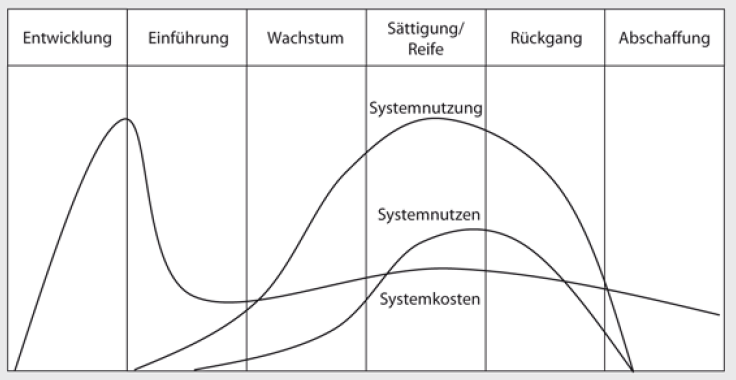
\includegraphics[scale=0.5]{Anwendungsleben.png}
      \end{minipage}
      
      
      
\end{itemize}


\vspace{0.5cm}
\subsection{Erstellung von Individualsoftware} %%%%%%%%%%%%%%%%%%%%%%%%%%%%%%%%%%%%%%%%%%%%%%%%%%%%%%%%%%%%%%%%%%%%%%%%%%%%%%%%%%
\begin{itemize}
   \item \textbf{Planung eines Softwareentwicklungsprozesses}:
      \begin{enumerate}
			\item Anforderungsanalyse und Erstellung einer Spezifikation
			\item Design
			\item Entwicklung
			\item Test und Integration
			\item Auslieferung des Produkts
			\item Wartung und Support
      \end{enumerate}
   
   \item \textbf{Strukturgetriebene Softwareentwicklung: Spiralmodell}\\
         Wiederholender Durchlauf von Entwicklungsphasen in Iterationen von jeweils 4 Schritten mit kontinuierlicher Bereitstellung von Prototypen.
      \begin{enumerate}
         \item \textbf{Analyse}:\\
                Definition von Rahmenbedingungen, Zielen, Anforderungen und Lösungsalternativen, Freigabe zur Umsetzung
         \item \textbf{Evaluierung}:\\
                Evaluierung der umgesetzten Lösungsalternativen. Darauf basierend Erkennung von Risiken und Erarbeitung adäquater Strategien zur Vermeidung der Risiken.
         \item \textbf{Realisierung}:\\
                Definition und anschließende Realisierung des Vorgehens, basierend auf den identifizierten Risiken.
         \item \textbf{Planung}:\\
                Review der vorangegangenen Schritte und Planung der nächsten Iteration
      \end{enumerate}
   
   \item \textbf{Prinzipien agiler Softwareentwicklung}:
      \begin{itemize}
			\item Transparenz und Geschwindigkeit der Entwicklung erhöhen\\
			      Reaktion auf Änderungen $>$ Verfolgung eines festgelegten Plans
			\item Fehler minimieren\\
			      Funktionierende Software $>$ Umfangreiche Dokumentation
			\item Kommunikation und Interaktion!\\
			      Kooperation mit Projektbetroffenen $>$ Vertragsverhandlungen\\
			      Individuen und Interaktionen $>$ Prozesse und Tools
      \end{itemize}
   
   \item \textbf{SCRUM}:
      \begin{itemize}
			\item Modell der agilen Softwareentwicklung
			\item Transparenz, Überprüfung und Anpassung
			\item Grober, zeitlicher Rahmen wird definiert und dann angepasst\\
			      $\rightarrow$ Sprint Planning
			\item Teams sind selbstorganisiert\\
			      $\rightarrow$  Scrum Master, Product Owner, Team\\
			      $\rightarrow$ Daily SCRUM Meetings
      \end{itemize}
   
   \item \textbf{DevOps}:
      \begin{itemize}
			\item Development + Operations
			\item \textbf{Ziel}: In sich verändernden Umgebungen mit schlanken und flexiblen Software-Entwicklungsprozessen schnell zu reagieren
			\item DevOpszur Integration von Entwicklung und Betrieb:
			\item[] 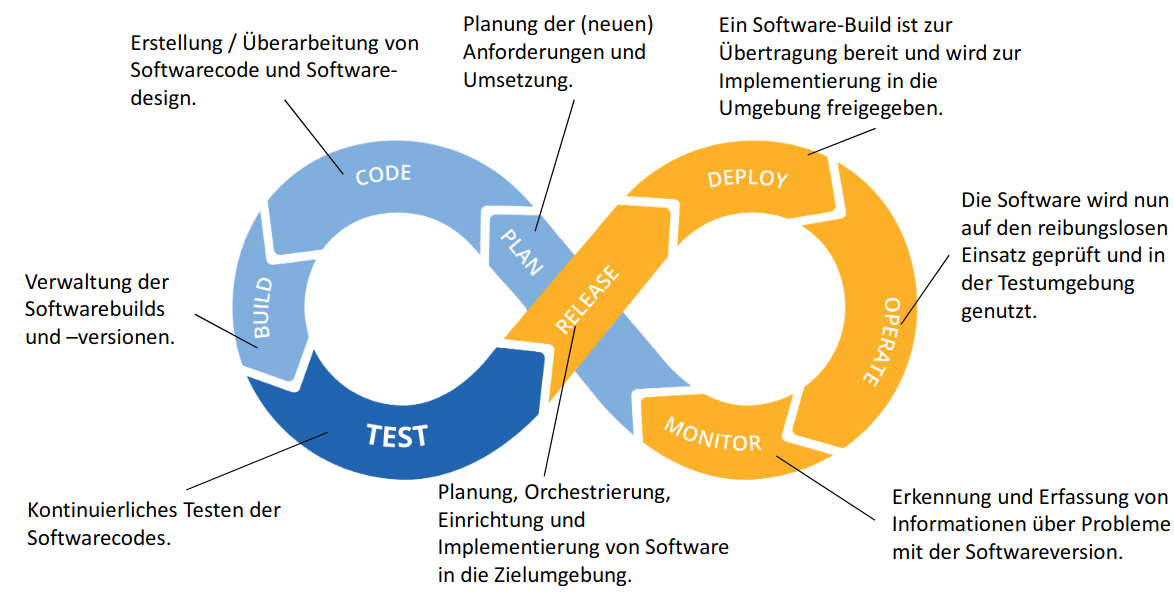
\includegraphics[scale=0.45]{DevOps.png}
			
			\item \textbf{Limitationen und Herausforderungen von DevOps}:
			   \begin{itemize}
					\item Flexibilität
					\item Automatisierung
					\item Lean-Prinzipien $\rightarrow$ System optimieren
					\item Alignment-Herausforderung $\rightarrow$ Überwachung der wichtigsten Indikatoren
					\item Kultur- und Wissensaustausch
            \end{itemize}
      \end{itemize}
   
   \item \emph{Magisches Dreieck} des Projektmanagements
   \item[] 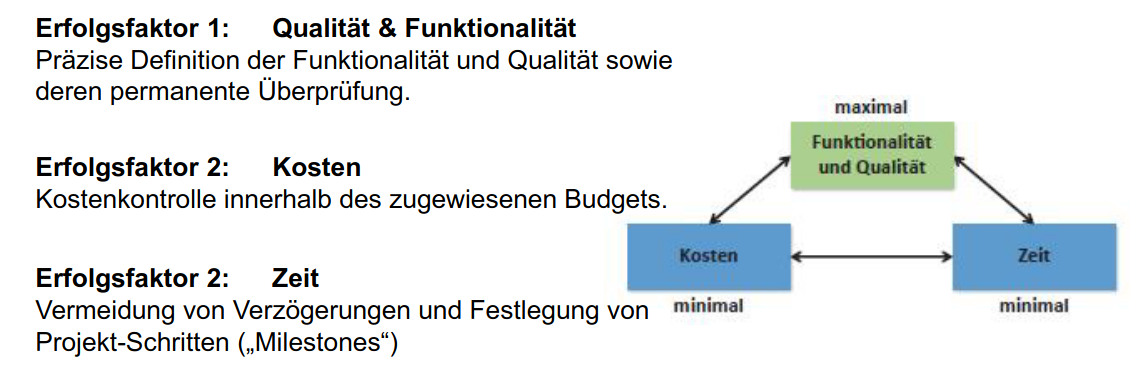
\includegraphics[scale=0.5]{magic.png}
\end{itemize}


\vspace{0.5cm}
\subsection{Beschaffung von Standardsoftware} %%%%%%%%%%%%%%%%%%%%%%%%%%%%%%%%%%%%%%%%%%%%%%%%%%%%%%%%%%%%%%%%%%%%%%%%%%%%%%%%%%%
\begin{itemize}
   \item \textbf{Vorgehen zur Softwareauswahl}:
      \begin{enumerate}
			\item Ist-Analyse
			\item Definition der Anforderung
			\item Marktanalyse
			\item Vergleich der Angebote
			\item Vertragsverhandlung
      \end{enumerate}
      
\newpage %Manuelle Formatierung
   \item \textbf{Kriterien für die Softwareauswahl}:
   \item[] 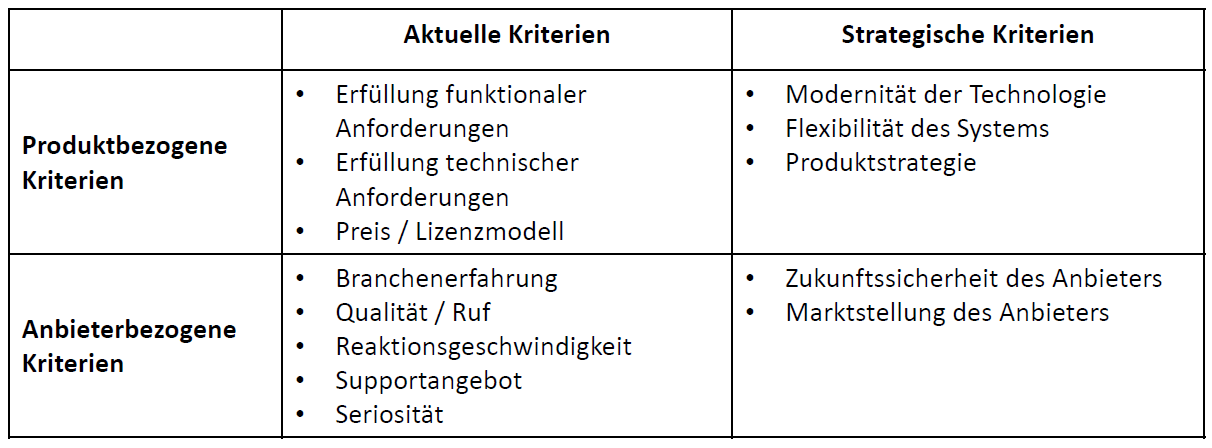
\includegraphics[scale=0.45]{KriterienSoftwareauswahl.png}
   
   \item \textbf{Proprietäre vs. Open Source Software}:
   \item[] 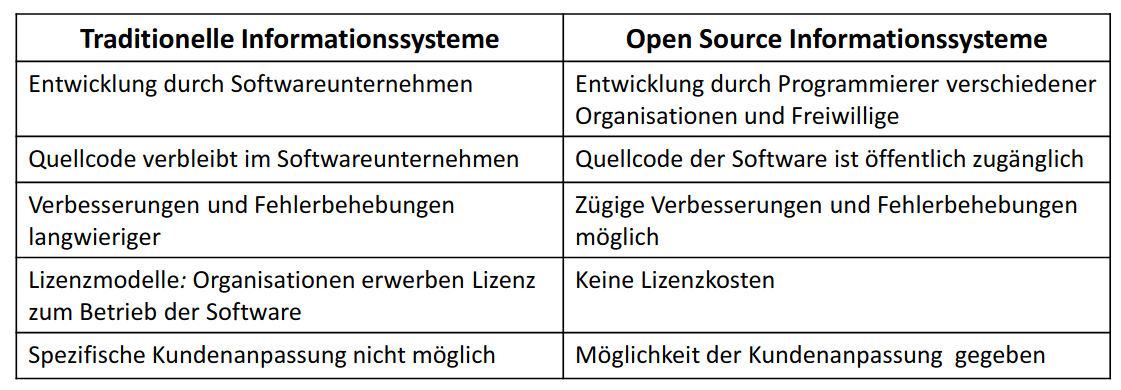
\includegraphics[scale=0.48]{foss.png}
   
   \item \textbf{IT-Outsourcing: Vor-und Nachteile}
   \item[] 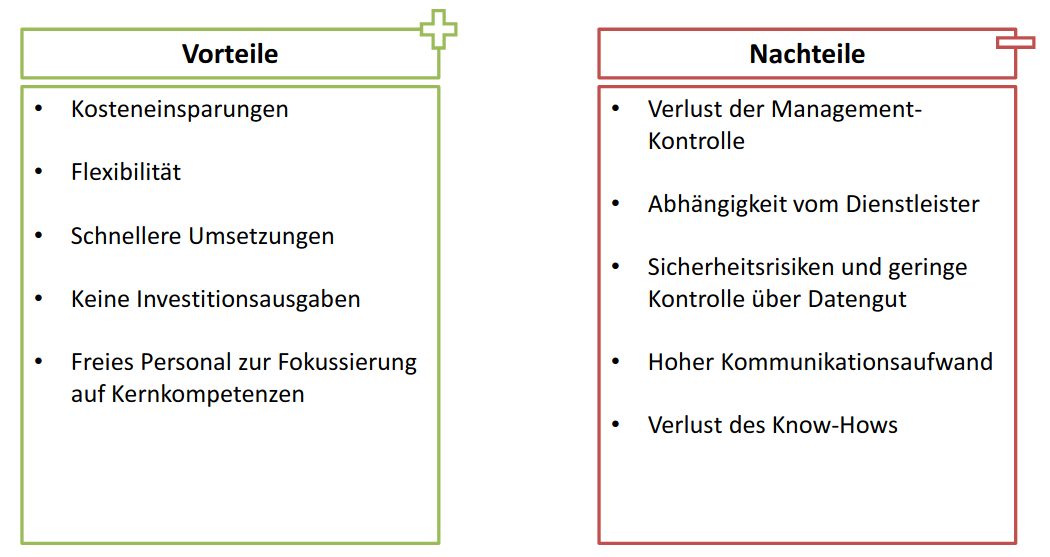
\includegraphics[scale=0.5]{out.png}
   
   \item \textbf{Cloud Computing}:\\
         Dynamische Bereitstellung von IT-Ressourcen über das Internet zur schnelleren Innovation und für flexiblere Ressourcen / Skaleneffekte
      \begin{itemize}
         \item \textbf{Infrastructure-as-a-Service (IaaS)}:\\
               Umfasst alle IT-Leistungen der Basisinfrastruktur z.B.Rechnerkapazitäten, Netzwerke und Speicherplatz.
         \item \textbf{Platform-as-a-Service (PaaS)}:\\
               IT-Leistungen, mit denen sich Anwendungssoftware und -komponenten entwickeln und integrieren lassen.
         \item \textbf{Software-as-a-Service (SaaS)}:\\
               Anwendungen und Dienste, die über Cloud Dienstebereitgestellt werden.
      \end{itemize}
\end{itemize}


\end{document}